\section{Experiment question, model, and objectives}
The experiment starts from the official \texttt{Qwen/Qwen2.5-0.5B} base, then applies SFT and DPO using the filtered educational data. The pinned revision begins \texttt{e332bac62ed3}; weights, tokenizer, and configuration have recorded hashes~\cite{qwenbase}. The model has 494,032,768 parameters and 24 Transformer layers. It is not the Instruct variant; Chapter~\ref{ch:agents}'s separately sourced Instruct diagnostic is not credited to this training. The research question is whether fitting demonstrations and optimizing pairwise preference improves generated teaching, assessed through matched questions and factual review.

LoRA freezes $W_0$ and learns $(\alpha/r)BA$ in query/value projections~\cite{lora}. Shared explicit ChatML serialization adds no system turn. Complete responses include the turn terminator; prompt and padding positions are masked, and selected training examples are not silently truncated. SFT minimizes response-token-normalized NLL:
\begin{equation}
\mathcal L_{\mathrm{SFT}}=-\frac1T\sum_{t=1}^T\log\pi_\theta(y_t\mid x,y_{<t}).
\label{eq:training-sft}
\end{equation}
DPO starts both policy and frozen reference from the selected SFT checkpoint. Reference sequence scores are cached before updates. With whole-response log probability $\ell_\pi$, preferred/dispreferred answers $y^+,y^-$ share the prompt:
\begin{align}
m_\theta&=\ell_{\pi_\theta}(y^+|x)-\ell_{\pi_\theta}(y^-|x)
-\bigl[\ell_{\pi_{\rm SFT}}(y^+|x)-\ell_{\pi_{\rm SFT}}(y^-|x)\bigr],\\
\mathcal L_{\mathrm{DPO}}&=-\log\sigma(0.1m_\theta).
\label{eq:training-dpo}
\end{align}
This relative objective~\cite{dpo} is not a factual-correctness score. Equal initial policy/reference predicts loss $\ln2$, supplying one integrity check alongside parent hashes and measured weight changes.

\section{Actual computation and model selection}
The historical CPU run uses an i7-12700H, approximately 16~GB RAM, six threads, and float32. It trains 128 SFT demonstrations and 64 preference pairs once, adapting the last four layers with $r=8$, $\alpha=16$ and 90,112 parameters. Learning rates are $8\times10^{-4}$ and $2\times10^{-4}$. All 15 original training families are represented; each stage uses 12.8\% of its released data. Both stages actually change weights. Its results remain separate because later experiments change the dataset and configuration together.

\begin{table}[H]\centering\small
\caption{Historical CPU results: complete references for 60 questions (13,437 response tokens); other measures use six greedy generations with a 192-token cap. Automatic unresolved labels are not factual errors.}\label{tab:training-cpu}
\begin{tabularx}{\linewidth}{@{}Yrrrr@{}}\toprule
Stage & Reference NLL & Automatic C/W/U & At cap & Repetition (\%)\\\midrule
Base & 3.276 & 0 / 0 / 6 & 6 & 44.9\\
SFT & 2.508 & 0 / 2 / 4 & 5 & 58.0\\
DPO & 2.664 & 0 / 0 / 6 & 6 & 72.8\\\bottomrule
\end{tabularx}
\end{table}\FloatBarrier

Both genuine cloud experiments use all 1,000 revised SFT examples over three epochs, 500 DPO pairs once, and a 500-update continued-SFT control from the same selected parent. They use float32, batch one, $r=16$, $\alpha=32$, seed 20261107, and DPO coefficient 0.1. The control uses the SFT split, not the chosen responses to the same DPO prompts; it matches updates and selected settings, not prompts, token counts, or strict compute.

\begin{table}[H]\centering\small
\caption{Recorded cloud configurations and development selection. Times sum optimization steps, excluding loading, reference caching, and evaluation.}\label{tab:training-protocol}
\begin{tabularx}{\linewidth}{@{}Yrr@{}}\toprule
Setting & First cloud run & Exploratory retry\\\midrule
Adapted Q/V layers & Last 8 & All 24\\
Trainable parameters & 360,448 & 1,081,344\\
SFT learning rate & $2\times10^{-4}$ & $1\times10^{-4}$\\
DPO / control learning rate & $1\times10^{-5}$ & $1\times10^{-5}$\\
SFT / DPO / control updates & 3000 / 500 / 500 & 3000 / 500 / 500\\
Dev NLL: epoch 1 & 2.6449 & 2.8672\\
Dev NLL: epoch 2 & 3.0709 & 3.3245\\
Dev NLL: epoch 3 & 3.3794 & 3.6293\\
Step seconds: SFT / DPO / control & 251.5 / 68.9 / 44.1 & 411.9 / 103.8 / 70.9\\\bottomrule
\end{tabularx}
\end{table}\FloatBarrier

Each run processes 143,934 SFT response tokens, 48,091 two-sided DPO tokens, and 23,981 control tokens. Complete-reference NLL on 36 development examples selects epoch one at 1,000 updates in both runs, preferring earlier epochs on ties. The 3,000-update SFT budget includes unselected epochs. Development covers only four coarse structures. Retry planning follows earlier test observations and simultaneously changes layer scope and SFT learning rate, so it is exploratory and cannot isolate either factor. The first package independently records CUDA but not the device name; retry Torch and \texttt{nvidia-smi} logs record T4 in both attempt records. Device logs are not external hardware attestation. 

\section{Paired outcomes and full-text review}
The fixed evaluation uses 24 Codex-authored natural questions, 100 held-out preference pairs, and 60 byte-preserved bridge references. Development records do not enter final metrics. All stages use identical prompts, greedy decoding, and a 384-new-token cap, preserving raw text, tokens, and stop reasons. NLL is token-weighted over complete references including terminators. Preference win proportion compares complete-sequence likelihoods and is length-sensitive, not human preference or student learning. The retry reuses an observed test rather than creating a new blind assessment.

Separate Codex reviewers read complete outputs, recording hashes, continuous evidence, interpretations, and reasons. A unique discernible primary claim matching execution is correct (C); a unique different claim is wrong (W). Missing answers, copied input, unclear roles, and unretracted conflicting claims remain unresolved (U). Explanation facts are checked separately. This is same-project, non-blind model-assisted review, not external teacher assessment.

\begin{table}[H]\centering\small
\caption{Matched cloud outcomes: 24 natural questions, 60 bridge references, and 100 preference pairs. EOS counts termination; C/W/U use full-text primary-output review. Preference and repetition columns are percentages.}\label{tab:training-cloud}
\begin{tabularx}{\linewidth}{@{}Yrrccrr@{}}\toprule
Stage & \shortstack{Natural\\NLL} & \shortstack{Bridge\\NLL} & \shortstack{EOS\\/24} & C/W/U & Pref. & Repeat\\\midrule
Base & 3.7258 & 3.2758 & 7 & 3/3/18 & 43 & 63.3\\
First SFT & 3.5892 & 4.0081 & 1 & 1/20/3 & 47 & 79.2\\
First DPO & 4.2992 & 4.5216 & 1 & 0/7/17 & 51 & 76.3\\
First control & 3.4445 & 3.9352 & 0 & 1/19/4 & 47 & 82.5\\
Retry SFT & 3.5873 & 4.2234 & 8 & 3/16/5 & 45 & 55.7\\
Retry DPO & 6.6152 & 6.7619 & 11 & 4/7/13 & 53 & 31.2\\
Retry control & 3.5764 & 4.3570 & 7 & 5/11/8 & 47 & 63.0\\\bottomrule
\end{tabularx}
\end{table}\FloatBarrier

First-cloud DPO worsens reference NLL on all 24 natural and 60 bridge items relative to SFT; continued SFT improves all 84 references but still fails to deliver reliable teaching. Retry SFT reduces repetition and ends more responses, while natural NLL changes only $-0.0019$ from first SFT. Retry DPO again worsens all 84 references despite preferred-sequence wins rising from 45\% to 53\% and EOS from 8 to 11. These endpoints do not support one aggregate claim of improvement.

\begin{figure}[H]\centering
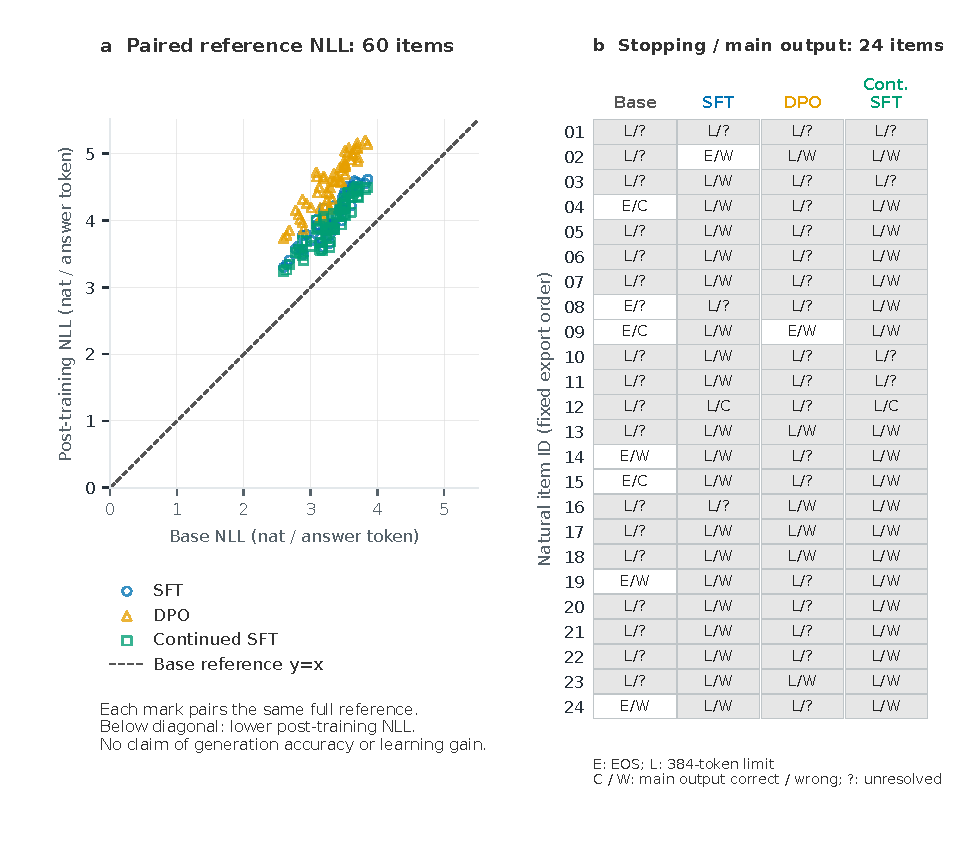
\includegraphics[width=\linewidth]{../../assets/en/training-v2-evidence.pdf}
\caption{First-cloud itemwise evidence: 60 paired bridge NLL values and 24 natural-question stopping/output records per stage. E denotes EOS, L the 384-token cap, and C/W/? full-text primary judgments; explanations are reviewed separately. All marks are recorded observations, with no seed-level significance claim.}\label{fig:training-v2-evidence}
\end{figure}\FloatBarrier

All three correct retry-SFT primary values have direct explanation errors. Of four correct retry-DPO values, three have false explanations and one is unclear. Of five correct control values, three explanations contain errors, one is unclear, and one has no identified factual error but still repeats severely. For example, SFT gives 11 for \verb|137 // 12| yet claims no remainder (the remainder is five); it gives 181 for \verb|[173,179,181,191][-2]| yet says negative indexing starts at zero. Correct values are therefore not complete teaching successes. The retry's 24 base responses exactly match the first run and reuse checked judgments; all 72 new trained responses are reviewed afresh.

\begin{figure}[H]\centering
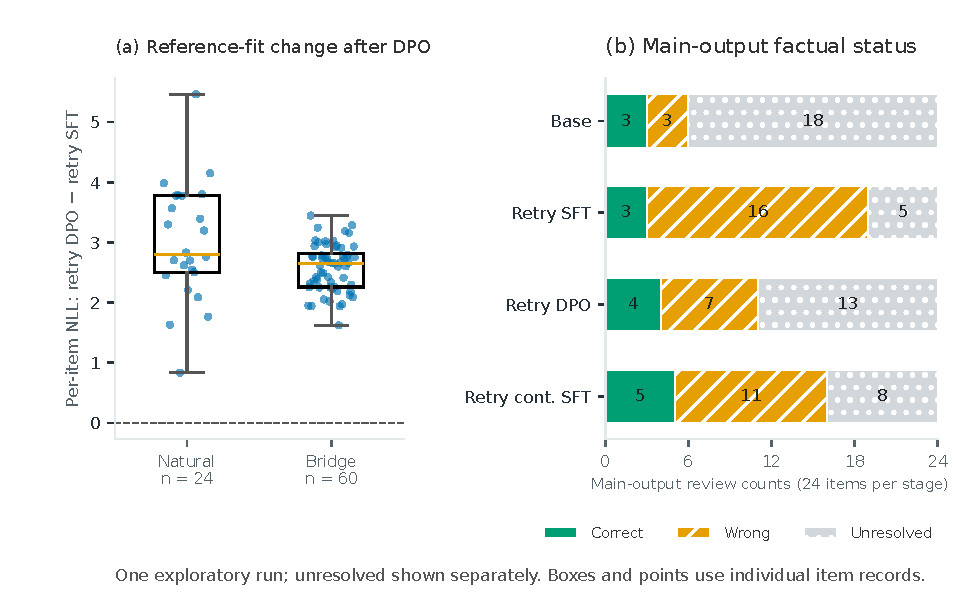
\includegraphics[width=\linewidth]{../../assets/en/training-retry-comparison.pdf}
\caption{Retry DPO-minus-SFT reference NLL and primary-output review. All 24 natural and 60 bridge items worsen in NLL; boxes summarize the recorded item distribution, not variability across training seeds. Unresolved remains distinct from wrong.}\label{fig:training-retry-comparison}
\end{figure}\FloatBarrier

\section{Two fixed questions: task, execution reference, and recorded behavior}
The following are the first two exported natural questions, fixed rather than selected for success. English excerpts translate recorded Chinese responses; ellipses mark omissions. Table judgments use the complete response, including contradictions absent from short excerpts. They are not new English generations or revised scoring rules.

\Needspace{25\baselineskip}
\subsection{NATURAL-01: assignment preserves an earlier value}
\begin{quote}\small
``I thought saved would decrease along with wallet. Can you tell me what is actually printed and explain what is wrong with that understanding?''
\begin{verbatim}
wallet = 137
saved = wallet
wallet = wallet - 18
print(saved)
\end{verbatim}
\end{quote}
Execution reference: \texttt{137}. Rebinding \texttt{wallet} does not change the integer value already bound to \texttt{saved}.

\begin{table}[H]\centering\small
\caption{Case 01: translated short excerpts and full-response primary judgments.}\label{tab:training-case01}
\begin{tabularx}{\linewidth}{@{}lYc@{}}\toprule
Stage & Recorded excerpt, translated & C/W/U\\\midrule
Base & ``It subtracts 18 from wallet and stores the result in saved.'' No unique original-program output. & U\\
First SFT & ``Output: 49'' \ldots\ ``Output: 101.'' & U\\
First DPO & ``Output: 79'' \ldots\ ``Output: 80.'' & U\\
First control & ``Output: 119'' \ldots\ ``the printed result is 117.'' & U\\
Retry SFT & ``Output: 119''; ``print(saved) outputs 119.'' & W\\
Retry DPO & ``Output 119'' \ldots\ ``Output: 18.'' & U\\
Retry control & ``Output: 119''; ``Passing wallet as an argument to -18 makes it [137].'' & W\\\bottomrule
\end{tabularx}
\end{table}\FloatBarrier

The failures concern assignment semantics rather than a missing output label alone. Repeated or competing values cannot be resolved by selecting a convenient number, including 137 copied from the prompt.

\Needspace{25\baselineskip}
\subsection{NATURAL-02: split, slice, and join}
\begin{quote}\small
``I am processing tree labels. Which names are sliced here? What text is finally joined together? Please explain directly using this example.''
\begin{verbatim}
label = 'oak|pine|elm|ash'
parts = label.split('|')
print('/'.join(parts[1:3]))
\end{verbatim}
\end{quote}
Execution reference: \texttt{pine/elm}. Indices 1 and 2 are selected; the joining separator is a slash.

\begin{table}[H]\centering\small
\caption{Case 02: code/output strings preserve original spelling; prose is translated.}\label{tab:training-case02}
\begin{tabularx}{\linewidth}{@{}lYc@{}}\toprule
Stage & Recorded excerpt, translated & C/W/U\\\midrule
Base & Repeats the full question and code, followed by ``erable''; no result is asserted. & U\\
First SFT & ``Output: /oak|pine|elm|ash''; the slice is said to retain oak and pine. & W\\
First DPO & ``Output: /amel|ash|elm|ash'' \ldots\ repeated \texttt{|ash}. & W\\
First control & ``Output: /oak|pine|elm|ash.'' & W\\
Retry SFT & ``Output: oak|elm''; ``keep only the first and third components.'' & W\\
Retry DPO & ``Output: oak|elm'' \ldots\ ``Output: ['oak', 'oak', 'elm', 'elm', 'elm'].'' & U\\
Retry control & ``Output: oak|elm''; ``remove the first and third semicolons.'' & W\\\bottomrule
\end{tabularx}
\end{table}\FloatBarrier

The original programs, complete requests, all seven stage outputs, stop reasons, and per-item reviews remain in \path{training/retry_imports/retry_048f9a92c0ef_numeric_review/comparison/} and the linked JSONs. Thus compact excerpts do not replace or silently discard negative evidence.

\section{Integrity exception, degradation, and the stopping decision}
The first cloud import passes 552 consistency checks. The initial retry import runs 965 checks and fails one first-step policy/reference threshold. Rejected-sequence scores differ by $1.52587890625\times10^{-5}$, one float32 representable step at that magnitude, whereas the old absolute threshold is $10^{-5}$; loss differs from $\ln2$ by $7.77\times10^{-7}$. The original failed audit is retained. A documented post-hoc review permits at most one step per sequence and checks ratios, margins, DPO scaling/loss arithmetic, and exact frozen-cache agreement. All 966 revised checks pass; boundary tests still reject larger or inconsistent discrepancies. A CPU probe does not reproduce the T4 reduction cause. This changes neither weights, outputs, nor factual labels and establishes internal consistency rather than effectiveness.

Inspection finds no obvious prompt-mask reversal, causal-shift error, omitted terminator, or truncation loss of the terminator. Development NLL worsens after epoch one. DPO saves only its final 500-step checkpoint, without intermediate development stopping; early stopping cannot be claimed retrospectively. Across the retry's steps 401--500, 96 of 100 pre-update training-pair snapshots score both responses below the frozen SFT reference; mean policy-minus-reference scores are $-37.761/-59.936$ nats. First-run values are 84 snapshots and $-8.550/-13.065$. Each snapshot concerns that step's pair, not a before/after measurement of one update or a fixed-set endpoint curve. These records show a larger relative preference margin alongside lower absolute likelihood; they do not isolate the cause of degraded generation. 

\paragraph{Observed limitations and possible causes.} The 1,000 SFT examples contain 145 coarse program structures; preference rejection reasons are coupled to task types, and the 36-item development set covers only four structures. Development NLL worsens after the first epoch, and the retry DPO reference NLL rises from 3.5873 to 6.6152 on the 24 natural questions. These observations indicate limited coverage and degraded reference fit, not their causes.

The small base model's capacity, narrow templates, preference shortcuts, and training choices could each contribute. No larger base was tested under the same protocol; the retry changes both layer scope and learning rate, and the continued-SFT control differs in prompts and token budget. Thus neither model size nor a single design choice can be assigned a causal share; overfitting remains a hypothesis. No additional training or model inference was performed.

\begin{figure}[H]\centering
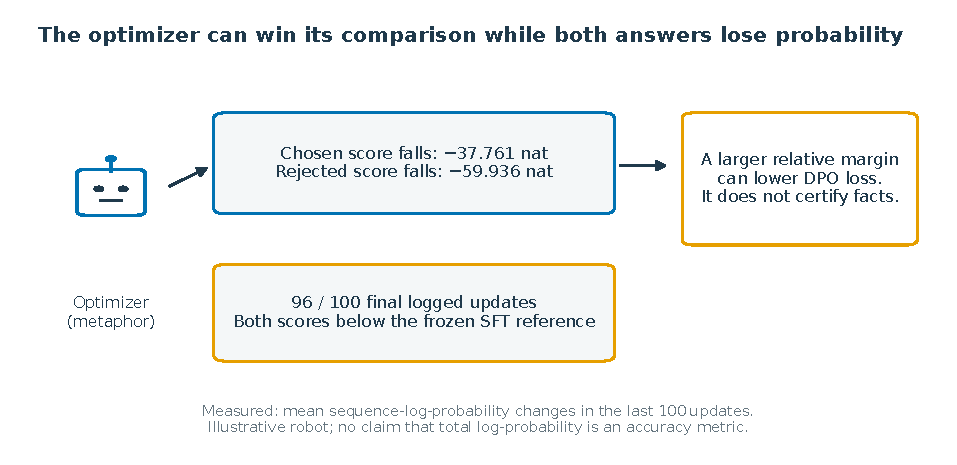
\includegraphics[width=\linewidth]{../../assets/en/training-objective-gap.pdf}
\caption{A relative preference objective can improve while both response probabilities fall. Values are pre-update, current-pair scores at steps 401--500 relative to frozen SFT, not changes caused by individual updates. The robot is a metaphor; sequence log probability is not accuracy or learning gain.}\label{fig:training-objective-gap}
\end{figure}\FloatBarrier

A single bounded local remedy, planned before its inference, mixes effective adapter updates rather than separately interpolating low-rank factors:
\begin{equation}
\Delta W_\lambda=(1-\lambda)\Delta W_{\mathrm{SFT}}+\lambda\Delta W_{\mathrm{DPO}}.
\end{equation}
No optimizer update occurs. All 36 development references select among fixed coefficients, preferring a smaller one for differences below $10^{-6}$.

\begin{table}[H]\centering\small
\caption{Bounded mixing on the development set. Zero is the SFT parent; one is complete DPO. This is post-hoc calibration, not a new blind training result.}\label{tab:training-remedy}
\begin{tabular}{@{}lrrrrr@{}}\toprule
$\lambda$ & 0 & 0.05 & 0.10 & 0.25 & 1\\
Development NLL & 2.8672 & 2.9447 & 3.0290 & 3.3237 & 5.9292\\\bottomrule
\end{tabular}
\end{table}\FloatBarrier

Zero wins, withdrawing DPO's increment within this family without repairing SFT. Six prespecified development cases then compare repetition penalties 1.0/1.08 with the same greedy 192-token cap. EOS improves from 1/6 to 3/6 and tokens fall from 970 to 717; each setting still has 0 correct, 4 wrong, and 2 unresolved primary outputs. Both report three \texttt{b}s where \texttt{aabbbbbab} has six; a loop with reference 112 receives 125 or 248. Competing Boolean claims remain unresolved. The development set is reused and has only four structures, so this is no independent validation.

The prespecified factual-failure stopping rule is met. The study ends at the recorded stopping decision: no further cloud training, test-set parameter search, or new deployment is performed. Broader data, cross-balanced preference reasons, intermediate checkpoints, and supervised anchoring remain unexecuted proposals. Complete answers, logs, numerical audits, and bounded-remedy results remain under \path{training/}. The result is a functioning SFT--DPO pipeline with poor teaching reliability, not a successful educational model.
